%To study the performance of Lazy Shadowing, we compare with process replication using the analytical models in Section~\ref{sec:analytical}. We also compare to checkpointing, of which the completion time is calculated with Daly's model~\cite{daly_fgcs_2006} and the energy consumption is then derived using Equation~\ref{eq:exp_energy1}. 
We compare with both process replication and checkpointing. %, assuming the same number of cores to use. 
The completion time with checkpointing is calculated with Daly's model~\cite{daly_fgcs_2006} assuming 10 minutes for both checkpointing and restart. The energy consumption is then derived with Equation~\ref{eq:exp_energy1}. It is important to point out that we always assume the same number of cores, so that process replication and Lazy Shadowing do not use extra cores for the replicas. 

It is clear from THEOREM 1 that the total recovery delay $\sum_{i=1}^k\tau_i$ is determined by the execution time $\sum_{i=1}^k\Delta_i$, independent of the distribution of failures. 
% which determines the individual value of $\Delta_i$. 
Therefore, our models are generic with no assumption about failure probability distribution, and the expectation of the total delay from all failures is the same as if failures are uniformly distributed~\cite{daly_fgcs_2006}. Specifically, $\Delta_i = w/(k+1)$, and $T_c^k = w + w*(1-\sigma_s^b)*\frac{k}{k+1}$. Further, we assume that each shadow gets a fair share of its core's execution rate so that $\sigma_s^b = \frac{1}{\alpha}$. %One may argue that the execution rate of the shadows
%should be degraded because of increased memory pressure or communication overhead. %Agreeing with that, however, we argue that 
%time sharing, which is the basic mechanism of multi-programming OS, is able to overlap computation and communication and improve system efficiency. For completeness, though, 
%To take that into account, we have also studied the slowing down effect using a penalty model, to be discussed later. 
To calculate Equation~\ref{eq:exp_energy2}, we assume that the dynamic power during shadow leaping is twice of that during normal execution, i.e., $p_{l}=2*p_d$, and the time for shadow leaping is half of the recovery time, i.e., $T_l=0.5*(T_{total} - w)$. %The static power ratio $\rho$ is fixed at 0.5 for our first study, other values are also studied in this section.

The first study uses $N=1$ million cores, %effectively simulating the future extreme-scale computing environment, and assumes that $W=1$ million hours. 
$W=1$ million hours, and static power ratio $\rho=0.5$.
For Lazy Shadowing we vary $\alpha$ from 1 to 10, understanding that it is unrealistic to collocate too many processes on a core. Besides $\alpha=1$, which is process replication, we only show $\alpha=5$ and $\alpha=10$ as others can be easily inferred from the figures.

\begin{figure}[!t]
	\captionsetup{justification=centering}
	\begin{center}
%		\subfigure[application fatal failure probability]
%		{
%			\label{fig:f3}
%			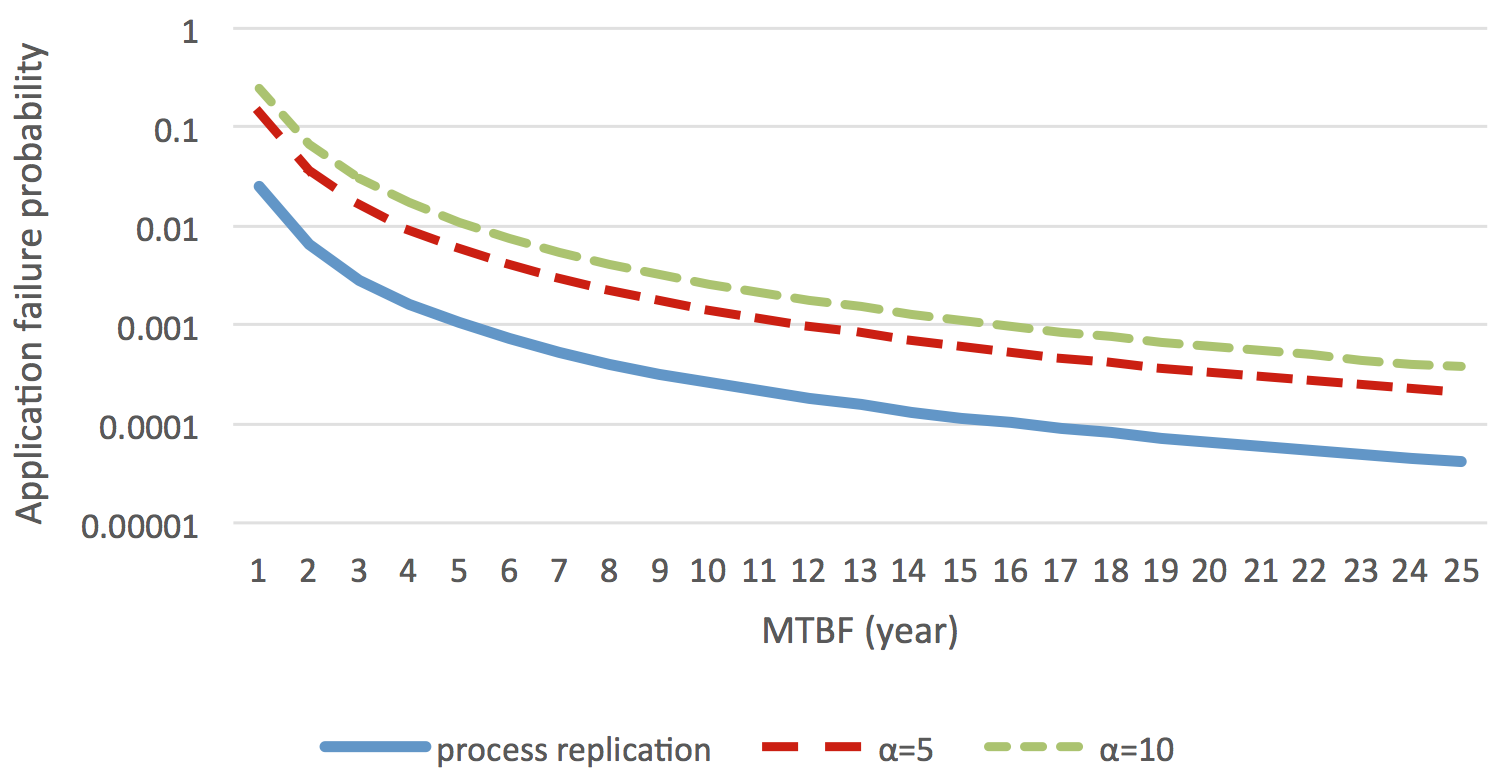
\includegraphics[width=0.7\columnwidth]{Figures/f3}
%		} 
%		\subfigure[Expected completion time]
%		{
%			\label{fig:t31}
%			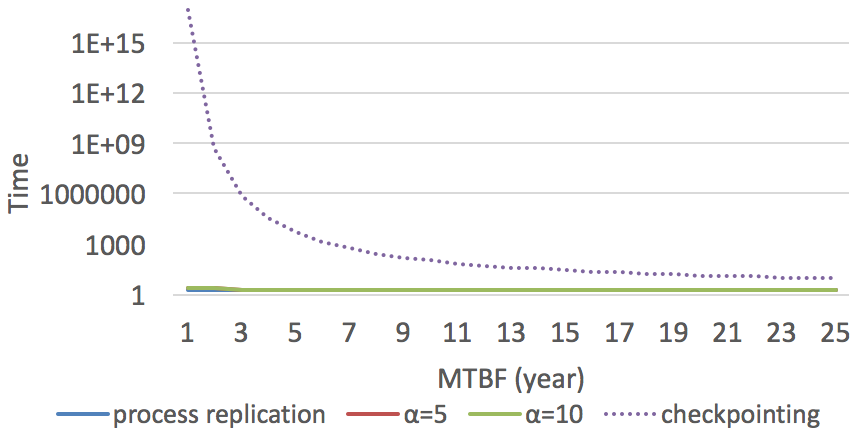
\includegraphics[width=0.7\columnwidth]{Figures/tt31}
%		} 
		\subfigure[Expected completion time]
		{
			\label{fig:t32}
			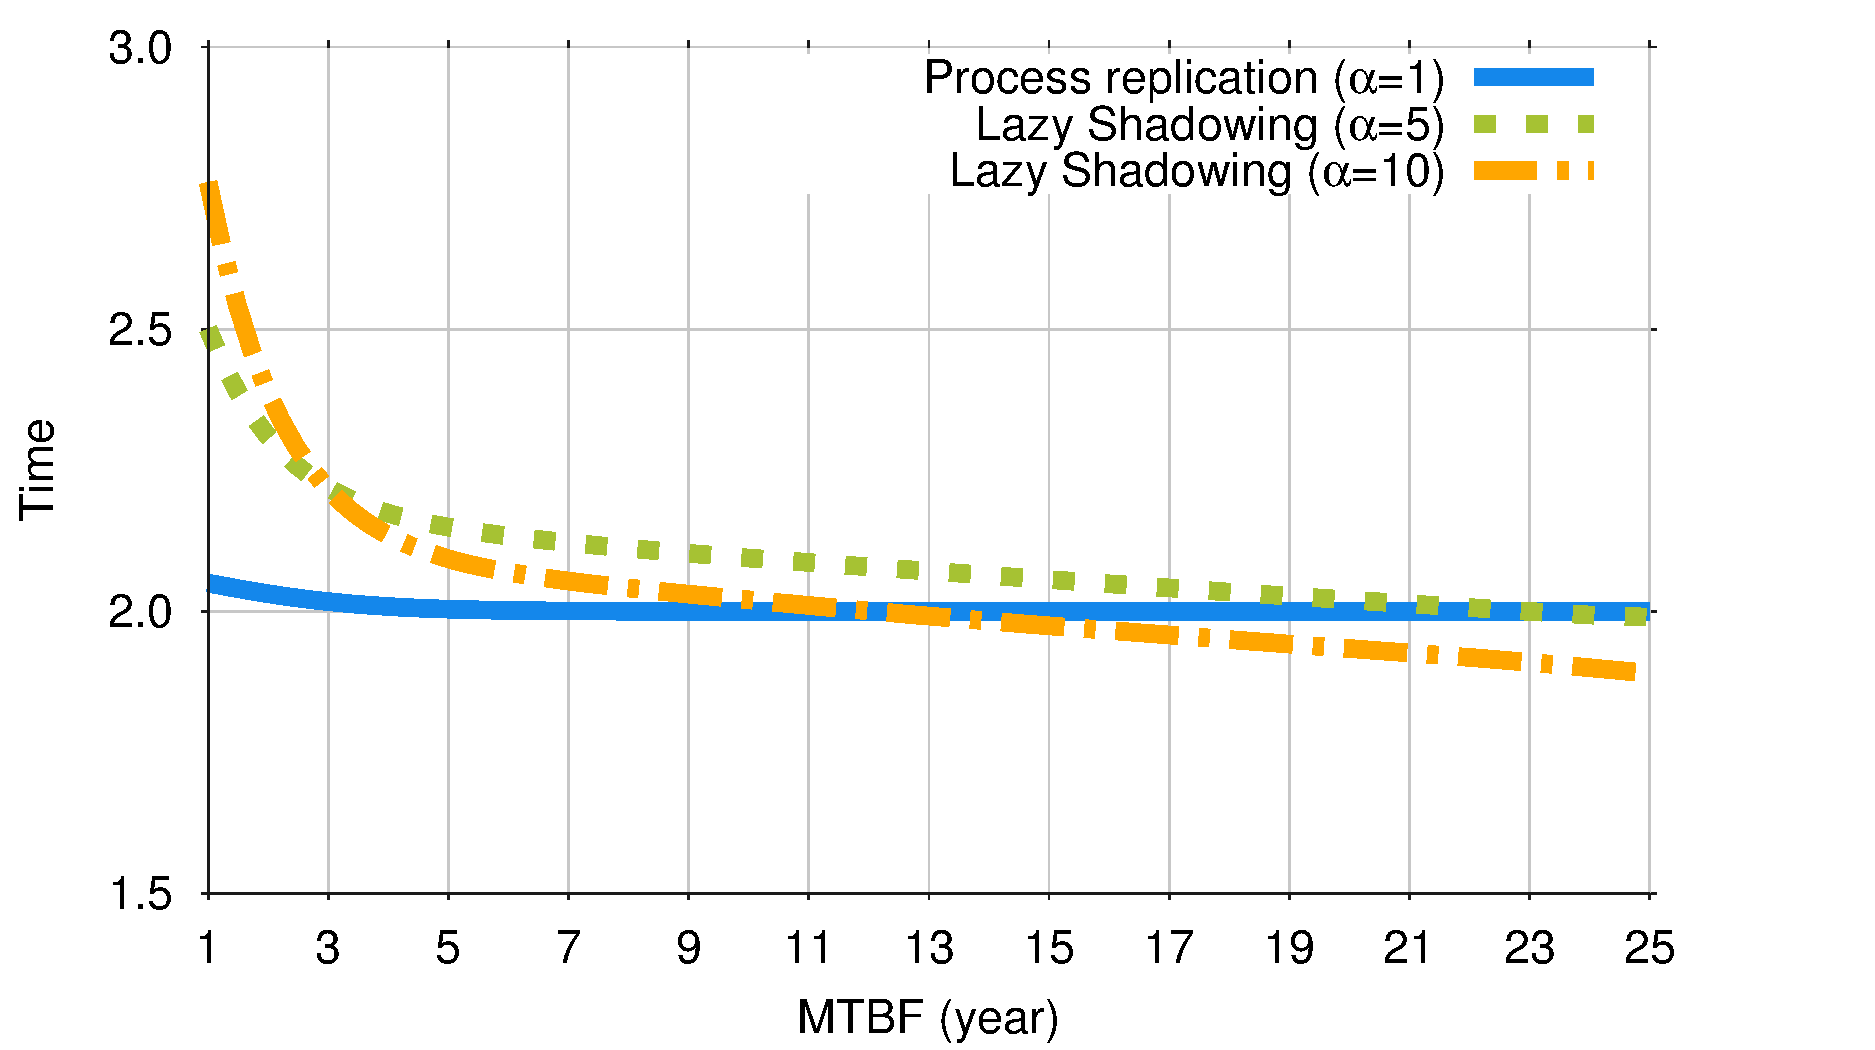
\includegraphics[width=0.7\columnwidth]{Figures/gen_time.pdf}
			%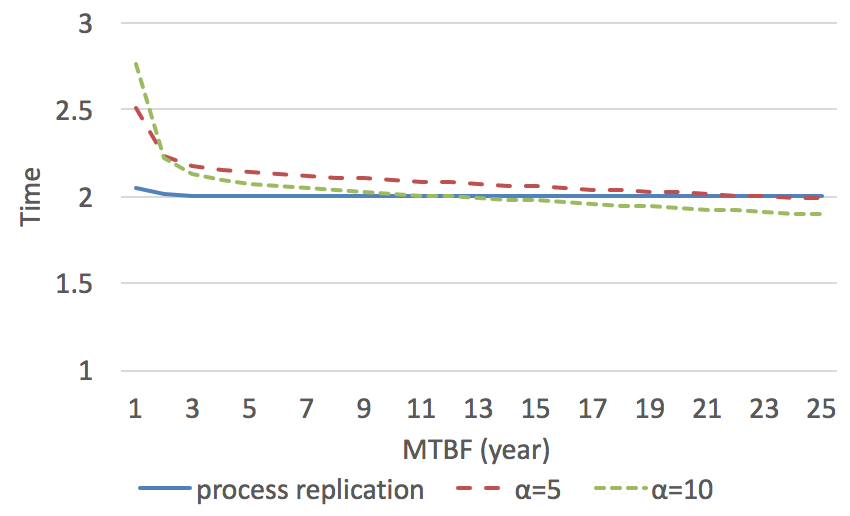
\includegraphics[width=0.7\columnwidth]{Figures/tt32}
		} 
		\subfigure[Expected energy consumption]
		{
			\label{fig:e32}
			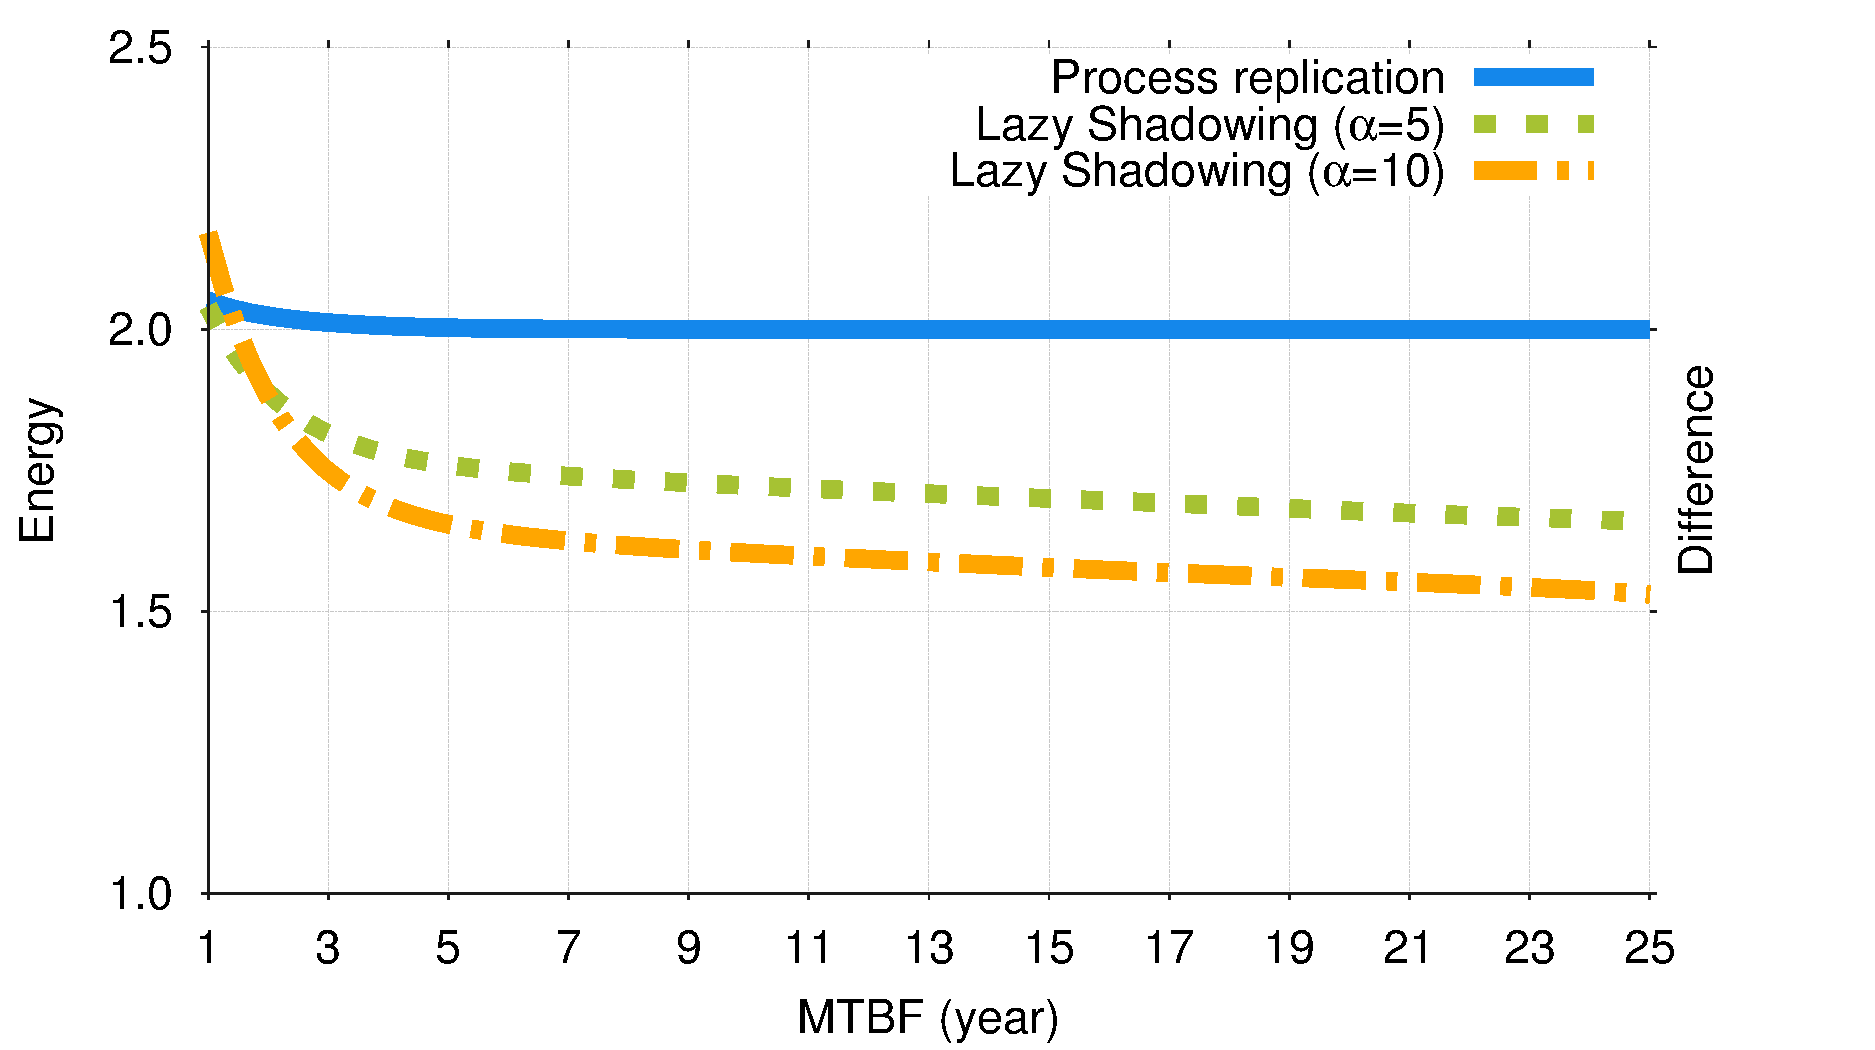
\includegraphics[width=0.7\columnwidth]{Figures/gen_energy.pdf}
			%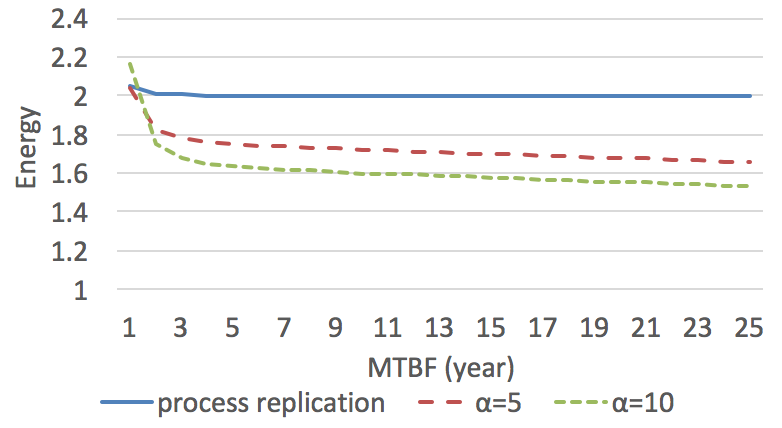
\includegraphics[width=0.7\columnwidth]{Figures/te32}
		} 
		\caption{Comparison of time and energy for different core level MTBF. $W=10^6$ hours, $N=10^6$, $\rho=0.5$.}
	\end{center}
	%\vskip -0.22in 
	\label{fig:3}
\end{figure}

%By definition, the application fatal failure probability for checkpointing is 0, as it periodically saves the execution states, from which the computation can be resumed upon failure. Figure~\ref{fig:f3} shows that due to collocation, the application fatal failure probability increases for Lazy Shadowing. 
We had a comprehensive study of the application fatal failure probabilities using models in Section~\ref{anal_app_fail}. Results show that application fatal failure probability increases slightly for Lazy Shadowing compared to process replication, as a result of shadow collocation (discussed in Section~\ref{sec:leaping_shadows}). However, even with unrealistically low MTBF of 1 year, Lazy Shadowing is still able to complete without rollback with greater than 0.75 probability. Therefore, we will not further discuss application fatal failure probability.  


%It is clear from Figure~\ref{fig:t31} that checkpointing incurs significant delay, indicating that it may not be a viable fault tolerance approach for future extreme-scale computing. 
Our results show that at extreme-scale, the completion time and energy consumption of checkpointing are orders of magnitude larger than those of Lazy Shadowing and process replication. Thus, we choose not to plot a separate graph for checkpointing in the interest of space. 
%so large that the comparison between process replication and Lazy Shadowing is invisible. Therefore, we re-plot the comparison between Lazy Shadowing and process replication in Figure~\ref{fig:t32} and~\ref{fig:e32}, with checkpointing removed. 
Figure~\ref{fig:t32} reveals that the most time efficient choice largely depends on MTBF. 
%More specifically, process replication consumes less time when MTBF is low while otherwise Lazy Shadowing is more efficient.
When MTBF is high, Lazy Shadowing requires less time as more cores are used for main processes and less workload is assigned to each process. As MTBF decreases, process replication outperforms Lazy Shadowing as a result of the increased likelihood of rollback for Lazy Shadowing.
%This is because of the increased probability of re-execution for Lazy Shadowing when failure rate is high. 
In terms of energy consumption, Lazy Shadowing has much more advantage over process replication. For MTBF from 2 to 25 years, Lazy Shadowing with $\alpha=5$ can achieve 9.6-17.1\% energy saving, while the saving increases to 13.1- 23.3\% for $\alpha=10$. The only exception is when MTBF is extremely low (1 year), Lazy Shadowing with $\alpha=10$ consumes more energy because of extended execution time.






